

\documentclass[preprint,12pt]{elsarticle}


\usepackage{amssymb}
%% The amsthm package provides extended theorem environments
%% \usepackage{amsthm}
\usepackage{hyperref}
\usepackage{amsmath}

\hypersetup{
    colorlinks=true, % 启用颜色链接
    citecolor=blue,  % 参考文献链接颜色设置为蓝色
    linkcolor=red,   % 内部链接(例如章节引用)颜色设置为红色
    urlcolor=blue    % 网络链接颜色设置为蓝色
    linkcolor=blue,    % 内部链接(例如图表和章节引用)颜色设置为蓝色
}
%% The lineno packages adds line numbers. Start line numbering with
%% \begin{linenumbers}, end it with \end{linenumbers}. Or switch it on
%% for the whole article with \linenumbers.
%% \usepackage{lineno}

\journal{Engineering Applications of Artificial Intelligence}

\begin{document}

\begin{frontmatter}


\title{Research on Comprehensive Human Emotion and Behavior Assessment System: Multimodal Emotion Recognition Combining Audio-Visual Inputs and Image Analysis Techniques for Behavioral Identification}


\author[a]{Xianxun Zhu}
\author[a]{Zhaozhao Liu}
\author[b]{Shoujin Wang}
\author[a]{Chaopeng Guo}
\author[a]{Heyang Feng}
\author[a]{Jingze Huang}
\author[a]{Rui Wang*}
\affiliation[a]{organization={School of Communication and Information Engineering, Shanghai University},
            addressline={No. 99, Shangda Road}, 
            city={Shanghai},
            postcode={200444}, 
            state={Shanghai},
            country={China}}
\affiliation[b]{organization={Data Science Institute, University of Technology Sydney},
            addressline={15 Broadway}, 
            city={Sydney},
            postcode={2007}, 
            state={Sydney},
            country={Australia}}

\begin{abstract}
With the rapid advancement of artificial intelligence and computer vision technologies, comprehensive assessment of human emotions and behavior has become a hot topic in contemporary scientific research. Traditional emotion recognition and behavior analysis often rely on single-modality data inputs, such as solely using images or audio. This approach often falls short in achieving desired accuracy and adaptability in complex real-world applications. To address this issue, we have developed a multimodal emotion recognition system that integrates audio and video inputs for a more comprehensive capture of subtle changes in human emotions. Additionally, we utilize advanced image analysis technology for behavior recognition, enabling a more accurate and in-depth understanding of human actions. Recognizing the inadequacies of existing emotion recognition technologies in practical multi-dimensional analysis, we have designed a novel multi-dimensional emotional and behavioral analysis model algorithm architecture. This architecture is capable of processing voice, text, images, and combinations of these modalities for conducting emotion analysis and behavior recognition. Experimental results demonstrate the significant effectiveness of our method in emotion and behavior recognition. Currently, specific emotional analysis applications lack a guiding architectural framework. Therefore, we have designed an end-to-end emotional and behavior recognition system, aiming to provide a new practical example for emotion and behavior recognition. This system is not only applicable in scenarios such as recommendation systems and abnormal emotion diagnosis but also offers new reference patterns for practical emotional applications. To facilitate the widespread deployment and application of this technology, we have made the detailed code available open-source at https://github.com/.

\end{abstract}

%%Graphical abstract
\begin{graphicalabstract}

\centering
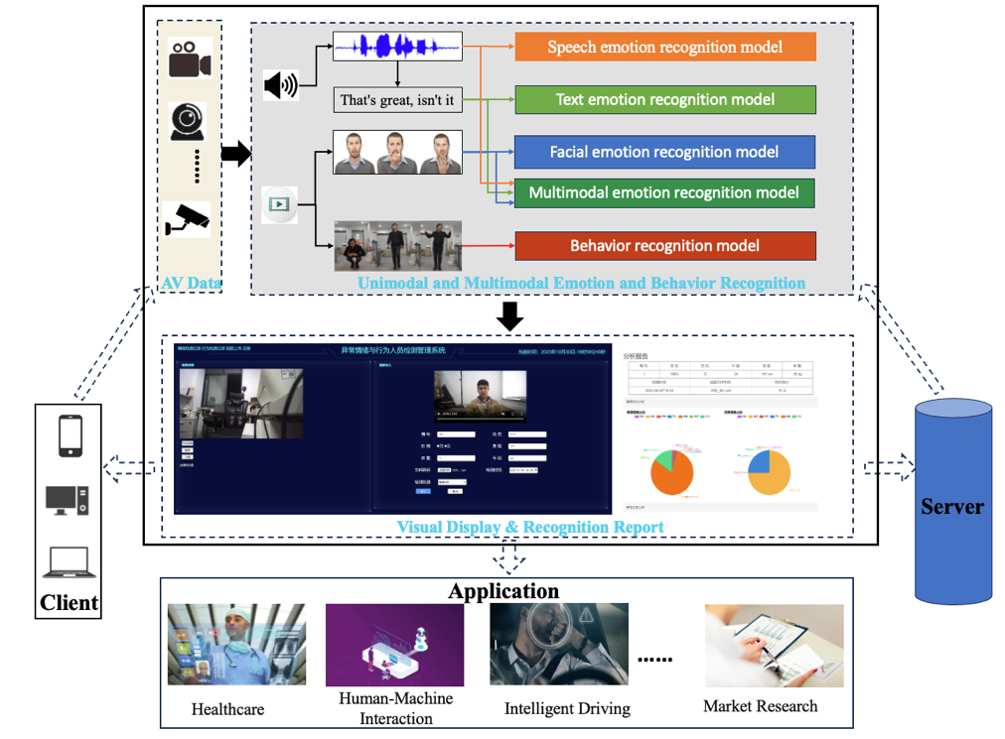
\includegraphics[width=1.1\textwidth]{Fig1.png}

\end{graphicalabstract}

%%Research highlights
\begin{highlights}
\item We present a novel multi-dimensional emotional and behavioral analysis model that integrates multimodal data (voice, text, images) to surmount current limitations in emotion recognition technology. Our experimental results demonstrate its high accuracy in comprehensive emotion and behavior analysis.
\item Introducing an innovative architecture, our model effectively processes and integrates multimodal data for enhanced emotion and behavior recognition accuracy, as validated by extensive experimental analysis.
\item Our research contributes a pioneering end-to-end system for emotional and behavior recognition, advancing the technological frontier and opening new avenues for practical applications in emotional analytics.
\item We have developed a unique mechanism for generating detailed emotion and behavior recognition reports, instrumental for applications like recommendation systems and abnormal emotion diagnosis. The decision to open-source our system's complete code underscores our commitment to its widespread adoption and ease of deployment.
\end{highlights}


\begin{keyword}
Multimodal, Emotion Recognition, Behavior Recognition, End-to-End System, Recognition Report.
\end{keyword}

\end{frontmatter}

%% \linenumbers

%% main text
\section{Introduction}
\label{}
In the fields of artificial intelligence and machine learning, emotion recognition and behavior analysis have emerged as key areas of research. With the advancement of technology, the need for multimodal emotion recognition and behavior analysis, particularly through audio and video inputs, is growing, demonstrating significant value in psychology, healthcare, and human-computer interaction \cite{ref1}. This study aims to develop a comprehensive human emotion and behavior assessment system, which combines audio and video inputs to accurately identify and assess an individual's emotional state and behavioral patterns through multimodal emotion recognition and image analysis techniques. Emotion recognition, especially through non-invasive methods like audio and video data analysis, offers a new perspective for understanding human emotions. The application of such technologies extends beyond fundamental scientific research into various aspects of everyday life, such as online education, smart homes, and autonomous vehicles. However, existing emotion recognition systems often rely on single-modality inputs, like audio or video alone, limiting their accuracy and applicability \cite{ref2, ref3}. On the other hand, behavior analysis holds significant importance in psychology and medical health. Image analysis techniques that monitor physical movements and behavior patterns are crucial for early diagnosis and treatment of various diseases \cite{ref4, ref5, ref6}.

In light of this, our study proposes an innovative comprehensive assessment system capable of processing both audio and video data, utilizing deep learning and image processing technologies for a holistic evaluation of human emotions and behaviors. Our goal is to enhance the accuracy of emotion recognition and behavior analysis and expand its potential applications across different fields. With this multimodal approach, we hope to gain a more comprehensive understanding of human emotions and behaviors, providing a more powerful tool for research and applications in related fields.

The innovation and workload of this study are primarily focused on the following four aspects:

\begin{itemize}
    \item Addressing the limitations of current emotion recognition technology in multi-dimensional analysis, we have developed a new multi-dimensional emotional and behavioral analysis model algorithm architecture. This architecture integrates and processes multimodal data such as voice, text, and images for comprehensive emotional analysis and behavior recognition. Our experimental analysis confirms the effectiveness and high accuracy of this model in emotion and behavior recognition.
    \item To tackle the issue of the lack of a clear guiding framework in existing emotional analysis applications, we designed an end-to-end emotional and behavior recognition system. This system not only fills a technological gap but also provides new application instances for emotion and behavior recognition.
    \item To delve deeper into the analysis of emotions and behavior recognition results, we have devised a mechanism for generating emotion and behavior recognition reports. These reports have significant application value and can be widely applied in scenarios like recommendation systems and abnormal emotion diagnosis.
    \item To promote the widespread application and convenient deployment of this technology, we have made the complete code open-source at https://github.com/zhuxianxun/Integrated-Human-Emotion-and-Behavior-Assessment-System.
\end{itemize}

\section{Related Work}
Current domestic and international research on emotion and behavior recognition primarily focuses on text emotion recognition, speech emotion recognition, image emotion recognition, multimodal emotion recognition, and image-based behavior recognition. This section briefly reviews the current state of research in emotion and behavior recognition.

\subsection{Facial Emotion Recognition}

Traditional facial emotion recognition technology mainly involves image preprocessing, feature extraction, and expression classification. However, as technology evolves and application scenarios expand, existing techniques face multiple challenges and limitations. In feature extraction, static and dynamic image processing methods each have their advantages and disadvantages. For instance, Gabor feature extraction  \cite{ref7} and Local Binary Patterns (LBP) \cite{ref8} perform well on static images, while feature point tracking and optical flow methods suit dynamic images. Despite this, challenges persist in processing time-series data. In emotion classification, existing methods like KNN, SVM, and random forests have their unique characteristics. For example, SVM excels with small-scale data but struggles with large-scale data processing. Deep learning methods, such as Convolutional Neural Networks (CNN) and Long Short-Term Memory networks (LSTM), have clear advantages in handling complex data but face issues like high model complexity and training difficulty \cite{ref9, ref10}.

\subsection{Text Emotion Recognition}

Text emotion recognition, a crucial research direction in natural language processing, has gained widespread attention in the international academic community in recent years. However, current research primarily focuses on emotion polarity analysis, with less attention to deep analysis of individual emotions. The basic task of emotion recognition is to identify the presence of emotion in the text, while emotion classification further analyzes specific emotion types within the text. Emotion recognition is important for narrowing the scope of emotion analysis and improving the performance of emotion classification. Researchers have utilized knowledge-based methods and machine learning technologies for emotion recognition on various corpora, such as Aman's work on blog articles and Maeda's research on Twitter datasets \cite{ref11, ref12}. These studies not only enhance emotion recognition accuracy but also offer new perspectives on emotion polarity and emotion category classification. Significant progress has also been made in constructing and applying Chinese emotion corpora, as demonstrated by Yao Yuanlin and others in the NLP\&CC2013 Chinese Weibo emotion analysis evaluation task \cite{ref13}, and Huang Lei's proposal of a syntax-based Weibo text emotion recognition method \cite{ref14}.

\subsection{Speech Emotion Recognition}

In traditional speech emotion recognition (SER) methods, SER is often viewed as a typical classification problem. Algorithms like Hidden Markov Models (HMM) \cite{ref15}, Gaussian Mixture Models (GMM) \cite{ref16}, Support Vector Machines (SVM), and Artificial Neural Networks (ANN) are widely used. These algorithms approximate mapping functions for emotion classification through training with labeled data and samples. Deep learning-based SER methods, such as CNN, RNN, LSTM, and attention-based techniques, have shown outstanding performance in the field. For instance, RNN and LSTM can process speech sequences in their entirety due to their sequential processing capabilities, making them more suitable for real-time emotion recognition scenarios. The CRNN structure, combining CNN and RNN/LSTM, is widely used to extract local and global emotional features of speech signals \cite{ref17}. Additionally, novel methods like 3D CNN, which extracts both short-term and long-term spectral features from speech signals, have significantly improved emotion recognition accuracy. These deep learning-based methods not only outperform traditional algorithms but also expand the application scope of speech emotion recognition \cite{ref18}.

\subsection{Multimodal Emotion Recognition}

A major challenge in multimodal emotion analysis and recognition tasks is the effectiveness of multimodal fusion strategies. Multimodal fusion mainly includes data-level fusion, decision-level fusion, and feature-level fusion. The aim of these methods is to utilize information from different modalities to enhance emotion recognition accuracy \cite{ref19}. Data-level fusion methods combine features at the raw data stage, learning feature representations directly from the raw data of various modalities \cite{ref20}. The challenge here is the differing data representations of each modality, making effective fusion complex. Feature-level fusion methods first extract useful features from the raw data of each modality, then further process and comprehensively analyze these features \cite{ref21, ref22}. This can address inconsistencies in raw data from different modalities and achieve a higher degree of information compression. Some studies have simply concatenated features from single-modality feature extraction stages, but this approach does not fully leverage the complementarity of different modalities in emotion analysis. Decision-level fusion methods, also known as late fusion, preprocess and extract features from each modality's data, inputting them into separate classifiers and then combining the results to obtain the final classification \cite{ref23}. This method is relatively simple but does not involve single-modality feature information and cannot fully utilize the original data. Beyond these explicit fusion methods, implicit methods like attention-based fusion have also been proposed. Recently, Transformer-based methods have been widely used, leveraging their attention mechanisms to learn dependencies between data from different modalities. These methods often consider the impact of different modalities on the final decision and the influence of long-term memory information on current emotions \cite{ref24,ref25}.

\subsection{Behavior Recognition}

Behavior recognition includes posture estimation and recognition phases. Human skeleton keypoint detection plays a foundational role in tasks like action classification and behavior recognition. For instance, the Hourglass network is a novel convolutional network architecture designed for human posture estimation. It processes human posture features at all scales, then merges them, capturing various spatial relationships related to the body \cite{ref26}. Its core lies in the combination of bottom-up, top-down processing, and intermediate supervision, greatly enhancing the network's performance. AlphaPose targets top-down keypoint detection algorithms. It addresses localization errors and duplicate detection issues in object detection processes and optimizes the detection of human bodies in different cropping areas using spatial transformer networks \cite{ref27}. HRNet, a popular model, consists of high-to-low-resolution subnets, repeatedly exchanging information between multi-resolution subnets. It maintains high-resolution feature information while extracting and fusing features of different sizes to provide rich semantic information \cite{ref28}. The classification of abnormal behavior recognition technology can be broadly divided into two categories: behavior recognition-based and anomaly detection-based \cite{ref29}. The former establishes abnormal posture samples and then discriminates specific behaviors through human target detection, posture estimation, and action recognition methods; the latter determines anomalies in videos based on similarity comparisons with normal scenes \cite{ref30}. Recently, the application of deep learning in abnormal behavior recognition has been increasing. For example, weakly supervised methods are used to detect abnormal behaviors in videos, dual-stream convolutional networks capture spatial and temporal information, and 3D CNNs extract video features. The key to abnormal behavior recognition lies in feature extraction, including methods based on human appearance and motion information, 2D human skeleton information, and deep learning-based feature extraction methods \cite{ref31, ref32}.
\begin{figure}[h]%
\centering
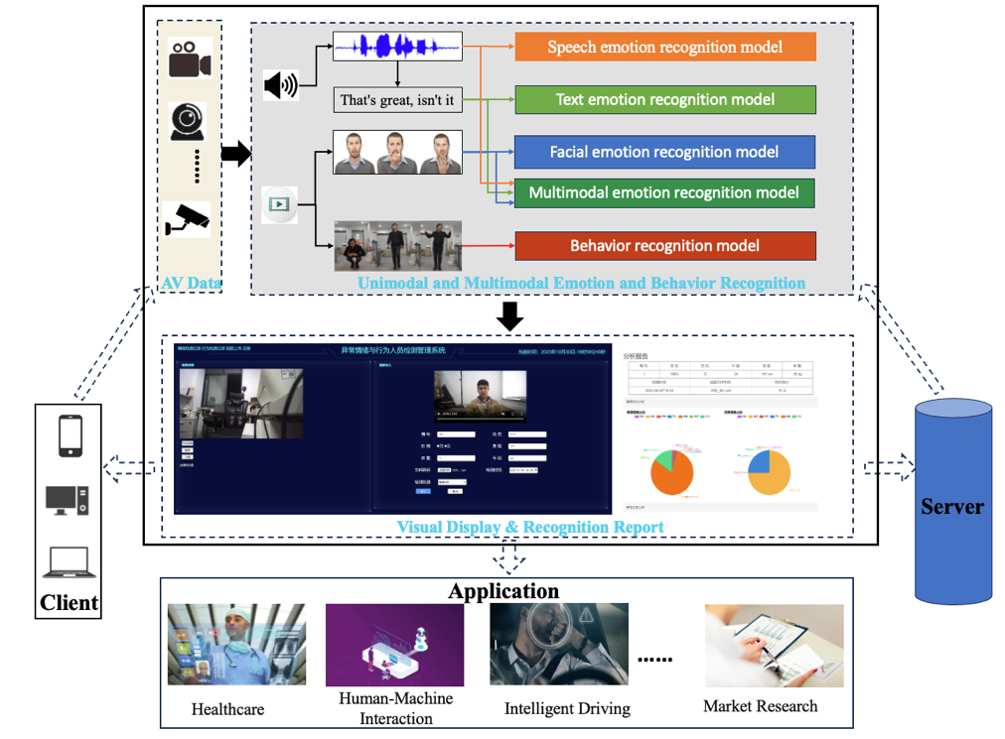
\includegraphics[width=1\textwidth]{Fig1.png}
\caption{Visual feature extraction block diagram.}\label{fig1}
\end{figure}
\section{Comprehensive Human Emotion and Behavior Assessment System}

This paper introduces an architecture for a comprehensive system designed to assess human emotions and behaviors, as depicted in Figure \ref{fig1}. The proposed architecture seamlessly integrates several key technologies and components. The client, initiating data collection, is tasked with acquiring audiovisual (AV) data, encompassing both images and audio. The system encompasses a suite of specialized algorithm models, including those for recognizing emotions in speech, text, and facial expressions, as well as multimodal emotion recognition and behavior recognition models. These models are trained offline and subsequently deployed on a server. At the server side, data received from the client undergoes processing through these algorithm models. This setup enables the recognition of emotions and behaviors in both single-modality and multimodal formats. The results of this analysis are then visually displayed on the front-end interface, offering users an intuitive and interactive recognition report. The utility of this system extends across various domains such as healthcare, human-computer interaction, intelligent driving, and market research, highlighting its wide applicability. In summary, this architecture effectively amalgamates diverse emotion and behavior recognition technologies, providing a robust and scalable solution for assessing human emotions and behaviors in a multitude of settings.




\subsection{Algorithm Models}

\textbf{Speech Emotion Recognition Model Based on DBN:} This model focuses on the recognition of emotions in speech, analyzing the emotional signatures embedded within voice signals. The intricacies of prosodic features necessitate a thorough examination of both intrinsic and statistical aspects of speech. This analysis isolates robust features pivotal for accurate emotion recognition. The primary step involves feature extraction, wherein five key aspects are derived from voice signals: pitch, short-term energy, short-term zero-crossing rate, formants, and Mel-frequency cepstral coefficients (MFCC) \cite{ref31}. 
\begin{equation}
Pitch Feature = \sqrt{\sum_{n=0}^{N-1}(s(n) - \bar{s})^2},
\end{equation}
where \( s(n) \) represents the signal deviation from its mean \( \bar{s} \), calculated over \( N \) samples. Subsequent investigations assess the interplay between these intrinsic features and their statistical properties, such as maxima, minima, means, variances, and standard deviations, to understand their contributions to emotion recognition.
\begin{equation}
Statistical Feature = \frac{1}{N}\sum_{i=1}^{N}x_{i}^{2},
\end{equation}
calculating the mean of the squared values of feature \( x_{i} \) over \( N \) observations.

Model Design and Optimization: The model synergizes Deep Belief Networks (DBN) with Support Vector Machines (SVM) within a multimodal emotion recognition framework \cite{ref32}. The Multimodal Affective Model is fine-tuned to precisely discern emotional states in Mandarin speech, demonstrating a high capability in processing feature vectors derived from deep neural networks.
\begin{equation}
Optimization= \arg\min_{W,b} \left\| H^v W_v + b_v - Y \right\|^2,
\end{equation}
striving to minimize the squared discrepancy between the model's predicted output \( H^v W_v + b_v \) and the actual output \( Y \). Hyperparameter Optimization: This crucial phase in model refinement involves the careful selection and tuning of parameters to optimize model performance \cite{ref33}. Model Training Acceleration: To enhance the efficiency of DBN training and conserve time, conjugate gradient methods are employed for fine-tuning parameter selection and adjustment.
\begin{equation}
Conjugate Gradient Method = W_{n+1} = W_n - \alpha_n \nabla F(W_n),
\end{equation}
where \( W_{n+1} \) denotes the updated parameters, \( W_n \) the current parameters, \( \alpha_n \) the learning rate, and \( \nabla F(W_n) \) the function's gradient subject to optimization.


\textbf{Speech Driven Text Emotion Recognition Model:} Our speech-driven text emotion recognition model employs an end-to-end approach, initially transforming speech signals into text through an encoder-decoder framework based on Recurrent Neural Networks (RNN). Specifically, the encoder RNN converts the input audio signals, represented as \( A \), into a fixed-length vector \( V \):
\begin{equation}
V = Encoder-RNN(A)
\end{equation}
where \( A \) denotes the input audio signals. The decoder network then transforms this vector \( V \) into a sequence of textual output \( T \):
\begin{equation}
T = Decoder - RNN(V)
\end{equation}
Incorporating attention mechanisms in the decoder greatly improves its ability to handle long audio inputs or to produce extended text outputs. The RNN encoder-decoder with attention mechanism shows superior performance in phoneme or grapheme level prediction tasks during the speech-to-text recognition process \cite{ref34}. We also integrate the Connectionist Temporal Classification (CTC) loss function with RNN to effectively model the temporal information in audio signals, allowing for variable-length input-to-output mapping:
\begin{equation}
CTC Loss = -\sum_{(x,y)\in \mathcal{D}} \log p(y|x)
\end{equation}
where \( \mathcal{D} \) is the dataset comprising pairs of input sequences \( x \) and their corresponding output label sequences \( y \). The CTC-RNN model excels in end-to-end speech recognition tasks, especially in generating text output at the grapheme level. Our approach forgoes traditional methods like frame-by-frame alignment using Gaussian Mixture Models-Hidden Markov Models (GMM-HMM) and using DNN cross-entropy networks for pre-training CTC-RNN networks, and instead opts for direct training of CTC-RNN networks from scratch, thereby streamlining the training process \cite{ref35}.

Advanced Text Emotion Analysis with Word Embedding: In our text emotion analysis, we utilize the advanced word embedding technology to convert vocabulary into continuous real-number vectors. Our choice of the BERT model, a pre-trained neural network-based model for natural language processing, marks a significant advancement over traditional word2vec language models due to its greater flexibility and capabilities \cite{ref36}. BERT distinguishes itself by dynamically adjusting word vector representations based on the context, thus enabling precise expressions for the different meanings of the same word in various contexts. This feature is essential in natural language processing, as it addresses the challenge of the same word having multiple meanings depending on the context \cite{ref37}.
\begin{equation}
Dynamic Word Vector_{BERT} = \sum_{i=1}^{N} ContextWeight_i \cdot WordEmbedding_i
\end{equation}
In this equation, \(ContextWeight_i\) represents the weight of the \(i^{th}\) word's contextual importance, and \(WordEmbedding_i\) is its initial embedding. This formula encapsulates BERT's ability to adjust word representations dynamically based on context.

The dynamic nature of BERT's word vectors enables them to capture a richer array of semantic features, leading to superior results in various natural language processing tasks, such as multi-task learning and QQP (Quora Question Pairs) \cite{ref38}. The enhanced quality of word vectors extracted from BERT provides a more enriched input for downstream tasks, significantly boosting the performance of models that rely on detailed language understanding.
\begin{equation}
\begin{aligned}
\text{Enhanced Model Performance} = \text{ActivationFunction} \bigg( \sum_{j=1}^{M} \text{VectorWeight}_j \cdot \\
\text{Dynamic Word Vector}_{BERT, j} \bigg)
\end{aligned}
\end{equation}
\textbf{Expression Recognition Model Based on Multi-Dimensional Feature Fusion and Self-Attention Mechanism:} We have developed a lightweight facial expression recognition model, utilizing attention mechanisms to address issues such as insufficient feature extraction and low accuracy in extreme environments. The model merges traditional facial expression recognition techniques with advanced deep learning methods, harnessing the power of geometric feature extraction and the ResNet18 network \cite{ref39}. 

Feature Extraction: The model marks and re-encodes keypoints, focusing on the eyebrows, eyes, and mouth. The geometric feature vectors are derived based on 68 key facial points. The feature vector computation is articulated as:
\begin{equation}
\text{Geometric Feature Vector} = \sqrt{\sum_{i=1}^{68} (\text{Euclidean Distance}(P_i, \bar{P}))^2}
\end{equation}
where \(P_i\) represents the coordinates of the \(i^{th}\) facial point and \(\bar{P}\) denotes the mean position of all points.
Deep Feature Extraction with ResNet18 Network: Deep emotional features are extracted using the ResNet18 network, leveraging its cross-layer connections and residual block design. The extraction process can be mathematically represented as:
\begin{equation}
\text{Deep Feature} = \text{ResNet18}(\text{Facial Image})
\end{equation}

Self-Attention Mechanism: The model effectively fuses geometric and deep features across dimensions using a self-attention mechanism, formulated as:
\begin{equation}
\text{Integrated Feature} = \text{Self-Attention}(\text{Geometric Feature Vector}, \text{Deep Feature})
\end{equation}
This mechanism calculates the correlations between different feature vectors to guide cross-dimensional feature interactions.

Expression Classification Module: The model combines global average pooling, fully connected layers, and classification functions to map the integrated feature information to predicted probabilities for each facial expression category, reducing model parameters while enhancing accuracy and stability. The integration of these advanced techniques allows our model to achieve superior performance in facial expression recognition \cite{ref40, ref41}.

\textbf{Multimodal Emotion Recognition Model Based on Self-Supervised Multi-Tasking:} We introduce an innovative end-to-end multimodal emotion recognition system, adept at integrating data from facial expressions, voice, and text. The model, embracing a self-supervised multi-task learning approach, concurrently trains on tasks involving both multiple and single modalities, achieving deep integration of information from each modality. This allows for the automatic transformation of speech to text in videos, bridging any gaps in textual information due to video inputs. The comprehensive model comprises preprocessing, feature extraction, modality fusion, and emotion classification stages. Initially, input data from each modality undergo preprocessing, which includes normalization, silence detection, and speech segmentation. Audio and visual data are then processed using Unidirectional Long Short-Term Memory Networks (Single-Directional LSTM) to extract temporal details and long-term dependencies \cite{ref42}. Feature extraction for each modality (text, audio, and visual) is then conducted to derive representative features, crucial for the fusion and classification processes that follow.

The Self-Supervised Multi-Task Emotion Fusion Network (MTME) lies at the heart of our model. It intricately combines multimodal tasks with single-modality tasks, capturing shared information across different modalities and highlighting each modality's unique attributes. For single-modality tasks, individual processing for text, audio, and visual modalities takes place \cite{ref43}, with each task yielding specific emotion analysis results. The model also includes a single-modality label generation module that crafts u-labels for these tasks, aiding in training and loss calculation.

Fusion of modalities involves a series of mathematical transformations:
\begin{equation}
Z_{fusion} = R_t \otimes R_a \otimes R_v
\end{equation}
\begin{equation}
Z'_{fusion} = \text{ReLU}(U_{z1} Z_{fusion} + c_{z1})
\end{equation}
\begin{equation}
e_m = U_{z2} Z'_{fusion} + c_{z2}
\end{equation}
In these equations, \(Z_{fusion}\) represents the initial fusion of features from textual (\(R_t\)), auditory (\(R_a\)), and visual (\(R_v\)) modalities. The matrices \(U_{z1}\) and \(U_{z2}\), along with their corresponding bias vectors, facilitate the transformation of the fused features. The emotion estimation \(e_m\) is then derived from this transformed fusion.

The model progresses to perform single-modality tasks for each of the textual, auditory, and visual modalities, generating individual emotion insights (\(e_t\), \(e_a\), and \(e_v\)). The uni-modal label generator then aligns these with the single-modal predictions to determine the loss.

The final classification leverages the multi-task fusion strategy. During training, the model simultaneously learns from the multimodal task as well as the three single-modality sub-tasks. The overall loss combines the losses from the multimodal task with those from the single-modal tasks:
\begin{align}
\text{Loss}_{total} &= \lambda \text{Loss}_m + \mu \text{Loss}_t + \nu \text{Loss}_a + \xi \text{Loss}_v \\
\text{where } \text{Loss}_m &= \frac{1}{N} \sum_{k=1}^{N} |e'_m - e_m| \\
\text{Loss}_i &= \frac{1}{N} \sum_{k=1}^{N} |e'_i - e_i| \quad \text{for } i = t, a, v
\end{align}
Here, \( \lambda \), \( \mu \), \( \nu \), and \( \xi \) are the weightings assigned to each loss component, balancing the contributions from multi-modal and single-modal tasks.

The model undergoes rigorous evaluation and optimization to ensure its effectiveness, typically involving testing on standard datasets and subsequent modifications based on the results. This model represents a significant advancement in the field of emotion recognition, harnessing the power of multimodal data and self-supervised learning to achieve nuanced understanding and accurate classification of emotional states.

\textbf{Behavior Recognition Network Model Based on Conditional Channel Attention Mechanism:} High-resolution is required for human posture estimation tasks to achieve high performance. The design of existing efficient networks often focuses on reducing the redundancy of matrix-vector multiplications while regulating loss while maintaining spatial information. Typical examples of this approach include classification networks like MobileNet and ShuffleNet. Additionally, encoder-decoder architectures and multi-branch architectures are widely used for optimizing spatial information processing \cite{ref45}. To further enhance efficiency, Conditional Channel Weighting Units are introduced to replace the costly pointwise convolutions in Shuffle blocks. These units perform cross-channel information exchange, significantly reducing computational complexity. Compared to traditional convolutional kernel weights, the weights in this scheme are conditioned on the input image and computed across channels through lightweight units, enabling effective information exchange. While maintaining high-resolution characteristics, the model undergoes pruning to reduce the number of layers in high-resolution branches. This step effectively lowers the model's complexity and computational load while maintaining accuracy in posture estimation. Furthermore, knowledge distillation techniques are employed to further optimize the model's performance \cite{ref46}. Weight computation in the model uses adaptive average pooling and 1×1 convolutions to generate partitioned weight maps through ReLU and Sigmoid functions. These weight maps become bridges for cross-channel and resolution information exchange. Each position's weight vector receives information from all resolution input channels, enabling effective information exchange between different resolutions. Homogeneous spatial weights are also computed at each resolution, depending on all pixels of the input channels at a single resolution and collected through global average pooling. The application of spatial weights allows every element in the output channels to receive contributions from all positions of all input channels. The proposed lightweight human posture estimation model performs excellently in terms of computational efficiency and performance. It effectively combines the advantages of high-resolution networks and the necessity of lightweight design, achieving efficient computation in resource-limited environments through innovative techniques and strategies.

\subsection{Interactive System}

Common online comprehensive personnel detection and assessment methods often rely on single-modality data. However, relying solely on one modality for emotion analysis can lead to confusion and misjudgment due to uncertainties like occlusions, lighting conditions, and disguises. Consequently, multimodal emotion recognition has gradually come into focus. By integrating assessments from multiple aspects, the accuracy of emotion classification has been significantly enhanced. Current multimodal feature fusion emotion recognition innovatively combines extracted features for comprehensive inference. Leveraging a Web management system, comprehensive personnel information management can be achieved. Visualization of personnel detection data allows for effective analysis of overall human states  \cite{ref60}. In response to the issues of single-method assessments and low accuracy in current personnel behavior and emotion evaluations, a management system combining various deep learning models for abnormal behavior and emotion detection has been designed and implemented. This management system, using a B/S architecture, allows access and operation across multiple platforms and devices. It relies on a browser for cross-platform operation, facilitating subsequent configuration and maintenance. The system development employs the Django backend framework, based on Python language, with a MySQL lightweight database for data storage \cite{ref47, ref48}. The frontend uses the Vue framework integrated with ECharts to construct the Web management system. This system utilizes multiple deep learning models to perform comprehensive state assessments, data visualization analyses, test report generation, and information management of target personnel.

\subsection{Emotion and Behavior Recognition Report}

The emotion and behavior state assessment reports designed in this study aim to provide users with comprehensive and in-depth psychological and behavioral analyses.

Emotion State Assessment Report: This report is dedicated to analyzing and interpreting users' emotional fluctuations and traits, covering a diverse range of emotions such as happiness, sadness, anger, and surprise. By meticulously analyzing emotional data across different time points and environmental contexts, the report reveals patterns and characteristics of users' emotional changes. Based on this, personalized emotion management suggestions are provided to help users achieve self-regulation and optimization of their emotions \cite{ref49}.






Behavior State Assessment Report: Focusing on users' behavioral patterns, this report encompasses multiple dimensions like activity frequency and behavioral habits. Through comprehensive observations and in-depth analyses of users' daily behaviors, the report reflects not only their habits but also reveals underlying behavioral patterns. This assists users in deeply understanding their personal behavioral traits and, when necessary, making reasonable behavioral adjustments.

\subsection{Model Training Datasets}

\textbf{Facial Expression Recognition Dataset}: FER2013 PLUS - This is an improved and optimized dataset based on FER2013. Due to non-facial data and inaccurate labels in FER2013, its facial expression recognition rate was only 65\%. To enhance the dataset's quality and effectiveness, researchers re-annotated FER2013, increasing the expression types to ten. Using the maximum voting method, some uncertain images were removed, making FER2013 PLUS more accurate and comprehensive. It contains 31,412 grayscale facial images, with 25,060 for training, 3,152 as a private test set, and 3,199 as a public test set \cite{ref50}.

\textbf{Speech Recognition Text Dataset}: CASIA - The chosen dataset is the Emotional Speech Dataset released by the Chinese Academy of Sciences, mainly used to evaluate the proposed speech recognition methods. The CASIA dataset is one of the most mainstream and widely used datasets in the field of speech recognition \cite{ref52}.

\textbf{Text Recognition Dataset}: THCHS-30 and SMP2020-EWECT - This dataset comprises two parts. The first part is the THCHS-30, an open-source Chinese speech dataset released by Tsinghua University, used for speech-to-text conversion. The second part is the SMP2020-EWECT, a Sina Weibo dataset provided by the Social Computing and Information Retrieval Research Center of Harbin Institute of Technology, covering six categories of Weibo texts. This part is primarily used for emotion recognition analysis of the converted text \cite{ref53, ref54}.

\textbf{Multimodal Emotion Recognition Dataset}: CH-SIMS - A novel Chinese multimodal emotion analysis dataset with independent single-modality annotations, suitable for both single-modality and multimodal emotion analysis. CH-SIMS includes 2,281 carefully selected real-life video clips with rich multimodal and single-modality annotations. This dataset is not only useful for studying interactions between different modalities but also applicable for emotion analysis based on single-modality annotations \cite{ref54}.

\textbf{Behavior Recognition Dataset}: For initial pre-training, the model utilizes the COCO public dataset  \cite{ref55}, which encompasses over 200,000 images and 250,000 instances of human figures. This dataset is well-suited for pre-training across a variety of computer vision tasks due to its extensive and diverse content. Subsequent validations are conducted on the Kinetics and Weizmann datasets to ensure the model's accuracy and efficacy in behavior recognition tasks  \cite{ref76}.


\section{Model Training Parameters}

\textbf{Facial Expression Recognition Model Experimental Setup}: Under the PyTorch deep learning framework, experiments were conducted in an Ubuntu 18.04 and Python 3.6 environment, utilizing 4 NVIDIA 1080Ti GPUs. Face detection and alignment were performed using MTCNN, followed by image cropping. Data augmentation and horizontal flipping were applied randomly. The experiments were conducted with a minimum batch size of 64, a fixed momentum of 0.9, and a dropout ratio of 0.5. Training was divided into two stages: the first stage started with a low learning rate for a total of 300 training epochs; the second stage had a learning rate of 1e-4, reduced by 0.1 every 20 epochs, for a total of 150 training epochs. The loss was optimized using stochastic gradient descent.

\textbf{Speech Emotion Recognition Model Parameters}: In the experiments, 39-dimensional MFCC features were extracted using the Librosa toolkit. Cross-entropy was used as the objective function, with a total duration of 500 epochs. The model was optimized with an initial learning rate of 0.001 and a batch size of 64. To prevent overfitting, label smoothing regularization with a factor of 0.1 was introduced. The model was evaluated using 10-fold cross-validation on 90\% training data and 10\% testing data to ensure fair comparison with state-of-the-art (SOTA) methods.

\textbf{Text Emotion Recognition Model Parameters}: Experiments were conducted using the PyTorch framework. After several adjustments, the final parameters were set to 30 epochs, a batch size of 64, a learning rate of 0.00001, and the Adam optimizer was chosen to achieve the highest model accuracy.

\textbf{Multimodal Emotion Recognition Model Parameters}: For audio processing, PCM 16-bit stereo encoding with a sampling rate of 44.1kHz was used. In video processing, the OpenFace tool was chosen, with a fixed frame rate of 25fps, and only a single face was processed. For text data processing, the pre-trained "bert-base-uncased" model was utilized. The output layer dimensions were 768 (text), 16 (audio), and 32 (video). During the training phase, data and model alignment were not performed, and normalization was disabled. An early stopping condition of 8 iterations was set, with the BERT model learning rate at 5e-5, and the audio and video parts set at 0.005. Weight decay parameters were differentiated for different parts.

\textbf{Behavior Recognition Model Training Parameters}: Training was conducted on a server equipped with 4 RTX3090 GPUs, with a batch size set to 64. Image preprocessing included fixing aspect ratios, cropping, resizing, and a series of data augmentation strategies. The Adam optimizer was used, with an initial learning rate set at 1e-3, reduced at specific epochs. Training terminated at the 210th epoch. The validation process included detecting the position of individuals and predicting human keypoints in two steps, using a posterior Gaussian filter to estimate heatmaps, and averaging predictions from original and flipped images.
%% The Appendices part is started with the command \appendix;
%% appendix sections are then done as normal sections
%% \appendix

%% \section{}
%% \label{}

%% If you have bibdatabase file and want bibtex to generate the
%% bibitems, please use
%%
%%  \bibliographystyle{elsarticle-num} 
%%  \bibliography{<your bibdatabase>}

%% else use the following coding to input the bibitems directly in the
%% TeX file.
\section{Model Performance Analysis}

\subsection{Baseline}

\textbf{Facial Expression Recognition Benchmark Models}: MobileNetV1 \cite{ref56}: A lightweight network suitable for mobile and embedded devices. FMPN \cite{ref57}: Feature Multi-Scale Fusion Network, effective in extracting features at different levels. ResNet18 \cite{ref58}: A kind of deep residual network, emphasizing deep feature learning. ShuffleNetV2 \cite{ref59}: An efficient lightweight network focusing on low computational cost. A-MobileNet \cite{ref56}: An improved version of MobileNet, enhancing accuracy and efficiency.

\textbf{Speech Emotion Recognition Benchmark Models}: DT-SVM \cite{ref61}: Decision Tree Support Vector Machine, combining the advantages of both methods. TLFMRF \cite{ref62}: Time-Frequency Multi-Scale Random Forest, capturing time-frequency features. GM-TCN \cite{ref63}: Graph Model Temporal Convolutional Network, emphasizing the processing of temporal data.

\textbf{Text Emotion Recognition Benchmark Models}: SVM \cite{ref64}: Support Vector Machine, a traditional baseline model for NLP tasks. TextCNN \cite{ref65}: The first convolutional neural network applied in the text domain. RCNN \cite{ref66}: Combining Recurrent Neural Network and Convolutional Neural Network to extract sequential and local text features. BiLSTM \cite{ref67}: Bidirectional Long Short-Term Memory network, focusing on text sequence features. BiLSTM-ATTN \cite{ref68}: Bidirectional LSTM with an added attention layer, enhancing feature extraction in significant areas.

\textbf{Multimodal Emotion Recognition Benchmark Models}: EF-LSTM \cite{ref69}: Early Fusion Long Short-Term Memory network, fusing features from different modalities for emotion analysis. LF-DNN \cite{ref70}: Late Fusion Deep Neural Network, processing single modality features separately before fusion and classification. TFN \cite{ref71}: Tensor Fusion Network, capturing interactions between different modalities through outer product operations. LMF \cite{ref72}: Low-Rank Multimodal Fusion, improving TFN by reducing model parameters.

\textbf{Behavior Recognition Benchmark Models}: Behavior recognition baselines include VGG+SSD \cite{ref73}, HOG+SVM \cite{ref74}, and DenseNet+SSD \cite{ref75}. VGG+SSD combines VGG's effective deep feature extraction with SSD's rapid object detection capabilities, ideal for identifying individuals and their actions. HOG+SVM leverages HOG's shape and texture descriptor with SVM's robust classification, effectively extracting and categorizing human behaviors. Lastly, DenseNet+SSD merges DenseNet's densely connected layers for enhanced feature retention with SSD's efficient detection, offering depth in feature understanding and performance in behavior recognition.
\subsection{Evaluation Criteria}

\textbf{Facial Expression Recognition Evaluation Criteria}: Accuracy (ACC) is commonly used as the metric to evaluate facial expression recognition systems. This metric reflects the overall performance of the model in classifying different facial expressions, calculated by comparing the model's predictions with the actual labels.

\textbf{Speech Emotion Recognition Evaluation Criteria}: Speech emotion recognition models typically use Weighted Average Recall (WAR) and Unweighted Average Recall (UAR) as performance metrics. WAR adjusts recall rates by category probability, considering the imbalance in sample sizes of categories, while UAR treats all categories equally, regardless of sample size differences. These two metrics jointly assess the model's recognition effectiveness across different emotional categories.

\textbf{Text Emotion Recognition Evaluation Criteria}: In text emotion recognition tasks, ACC and F1-score are primarily used to evaluate model performance. Accuracy directly reflects the model's accuracy in classifying emotional categories, while the F1-score, a harmonic mean of precision and recall, comprehensively assesses the model's performance across different categories.

\textbf{Multimodal Emotion Recognition Evaluation Criteria}: This task uses Binary Classification Accuracy (Acc-2) and F1-score as key evaluation metrics. Additionally, Mean Absolute Error (MAE) measures the accuracy of predictions; a lower MAE indicates higher model performance. Correct recognition rates are also used in practical tests to assess the overall efficacy of the model.

\textbf{Behavior Recognition Evaluation Criteria}: The field of behavior recognition commonly uses the accuracy of abnormal behavior recognition as an evaluation standard. This metric reflects the model's accuracy in predicting behavior categories, i.e., the proportion of the model's first prediction (the highest probability prediction) that matches the actual label. High accuracy implies better performance in recognizing different behaviors and is a commonly used performance metric for behavior recognition systems.


\subsection{Performance Results}

\textbf{Facial Expression Recognition Outcomes}: As shown in Table \ref{Table1}, it is evident that the "Ours" model achieves an accuracy of 91.30\%, which is significantly higher than other commonly used models such as MobileNetV1 (85.40\%), ResNet18 (87.37\%), and A-MobileNet (88.11\%). This indicates that the "Ours" model possesses superior accuracy and reliability in the task of facial expression recognition.
\begin{table}[ht]
\centering
\caption{Facial Expression Recognition Model Performance Comparison}\label{Table1}
\begin{tabular}{lc}
\hline
Method              & Accuracy (\%) \\
\hline
MobileNetV1         & 85.40        \\
MobileNetV2         & 77.18        \\
MobileNetV3         & 73.24        \\
FMPN                & 73.40        \\
ResNet18            & 87.37        \\
ShuffleNetV2        & 86.77        \\
A-MobileNet         & 88.11        \\
Ours                & 91.30        \\
\hline
\end{tabular}
\end{table}

\textbf{Speech Emotion Recognition Results}: As shown in Table \ref{Table2}, it can be observed that our model, "Ours," achieved a performance of 91.08\% in both Unweighted Average Recall (UAR) and Weighted Average Recall (WAR) on the CASIA dataset. This performance surpasses previous models such as DT-SVM (85.08\%), TLFMRF (85.83\%), and GM-TCN (90.17\%). This indicates that the "Ours" model demonstrates higher accuracy and reliability in speech emotion recognition.
\begin{table}[ht]
\centering
\caption{Results of Speech Emotion Recognition}\label{Table2}
\begin{tabular}{lcc}
\hline
Model       & UAR (\%) & WAR (\%) \\
\hline
DT-SVM  & 85.08    & 85.08    \\
TLFMRF & 85.83    & 85.83    \\
GM-TCN& 90.17    & 90.17    \\
Ours          & 91.08    & 91.08    \\
\hline
\end{tabular}
\end{table}

\textbf{Text Emotion Recognition Results}: As shown in Table \ref{Table3}, the "Ours" model achieved an accuracy of 77.20\% and a Macro-F1 score of 74.40\%, surpassing all other models listed. This highlights the outstanding performance of the "Ours" model in the field of text emotion recognition, particularly in terms of accurately classifying and balancing performance across various categories.
\begin{table}[ht]
\centering
\caption{Comparison of Text Emotion Recognition Model Experimental Results}\label{Table3}
\begin{tabular}{lcc}
\hline
Model           & Accuracy (\%) & Macro-F1 (\%) \\
\hline
SVM             & 69.10         & 63.60         \\
TextCNN         & 75.90         & 72.20         \\
RCNN            & 73.40         & 68.30         \\
BiLSTM          & 75.10         & 71.30         \\
BiLSTM-ATTN     & 75.60         & 71.40         \\
BERT            & 75.80         & 71.60         \\
BERT+BLS        & 76.10         & 72.00         \\
BERT+CFBLS      & 76.20         & 72.10         \\
BERT+CEBLS      & 76.50         & 72.30         \\
BERT+CFEBLS     & 76.30         & 72.40         \\
Ours            & 77.20         & 74.40         \\
\hline
\end{tabular}
\end{table}

\textbf{Multimodal Emotion Recognition Results}: As shown in Table \ref{Table4}, our model "Ours" demonstrates leading performance across several key metrics. Specifically, it achieved 77.9\% in Binary Classification Accuracy (Molt acc 2) and 78.19\% in F1 Score, both higher than other models like EF-LSTM, LF-DNN, LMF, and TFN. This indicates a clear advantage of the "Ours" model in terms of accuracy and balanced performance. Lowest Error: The "Ours" model scored 40.95 in Mean Absolute Error (MAE), the lowest among all models, signifying its superiority in prediction accuracy. A lower MAE implies that the model's emotion predictions are closer to the actual situation. High Correlation: With a score of 59.95 in the Correlation (Corr) metric, the "Ours" model exhibits the highest correlation, meaning that its predictions are most strongly correlated with the actual data. This reflects the model's capability to understand and capture emotional data. Loss Analysis: Although the "Ours" model's performance in the Loss aspect is slightly higher than other models, considering its significant advantages in other key performance indicators, this loss can be seen as a reasonable trade-off between model complexity and performance optimization.
\begin{table}[ht]
\centering
\caption{Comparison of Multimodal Emotion Recognition Model Experimental Results}\label{Table4}
\begin{tabular}{lccccc}
\hline
Model   & Molt acc 2 (\%) & F1 Score (\%) & MAE & Correlation & Loss \\
\hline
EF-LSTM & 76.42           & 75.83         & 44.53 & 57.04      & 43.76 \\
LF-DNN  & 77.45           & 77.58         & 44.46 & 57.68      & 43.35 \\
LMF     & 75.34           & 76.44         & 44.88 & 56.17      & 41.32 \\
TFN     & 76.65           & 77.92         & 41.66 & 58.23      & 41.22 \\
Ours    & 77.90           & 78.19         & 40.95 & 59.95      & 44.96 \\
\hline
\end{tabular}
\end{table}

Analyzing Table \ref{Table5}, our model demonstrates exceptional performance in Abnormal Behavior Recognition, particularly against the Kinetics and Weizmann datasets. With an 87.4\% accuracy on Kinetics and 94.5\% on Weizmann, it significantly outperforms models like VGG+SSD, HOG+SVM, and DenseNet+SSD. This high precision across datasets highlights the robustness and effectiveness of our approach. Notably, our model exceeds the DenseNet+SSD's 85.1\% accuracy on Kinetics and 90.2\% on Weizmann, showcasing its superior ability in identifying and categorizing abnormal behaviors. This versatility and precision mark a new standard in the field, demonstrating the model's potential for real-world applications where accurate abnormal behavior detection is essential. The model's success is attributed to its advanced, fine-tuned algorithmic structure, which captures the subtleties of abnormal behavior more effectively than existing models.
\begin{table}[h]
\centering
\caption{Comparative Performance of Abnormal Behavior Recognition Models}\label{Table5}
\begin{tabular}{lcc}
\hline
Model & Accuracy (\%)(Kinetics) & Accuracy (\%)(Weizmann) \\
\hline
VGG+SSD & 77.3 & 86.6 \\
HOG+SVM & 78.9 & 88.7 \\
DenseNet+SSD & 85.1 & 90.2 \\
Ours & 87.4 & 94.5 \\
\hline
\end{tabular}
\end{table}

\subsection{ Interaction System and Diagnostic Reporting}

A range of functionalities has been implemented through the integration of a camera system, including the recording, playback, and downloading of video files. Specifically, users can capture real-time footage using the camera, subsequently generating video files. These files can be played back directly within the system or downloaded to local devices for further use. Additionally, the system features a specially designed interface for the entry of subject information, as well as the collection and recording of video data, as illustrated in Figure \ref{fig2}.

\begin{figure}[h]%
\centering
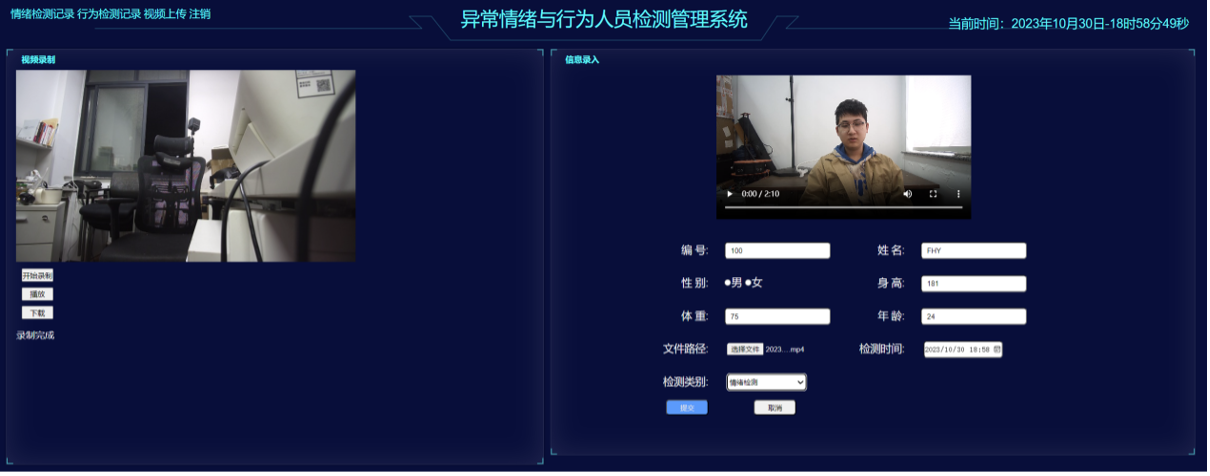
\includegraphics[width=1\textwidth]{Fig2.png}
\caption{Personnel Detection Information Entry and Video Recording Preservation.}\label{fig2}
\end{figure}

In the information entry interface, users can fill in basic details of the subjects such as name, age, and gender, ensuring accurate correspondence and documentation of video data with personal information. During the video data collection and recording phase, users can initiate the camera with simple operations for real-time monitoring and recording of subject activities. This process is not only efficient but also user-friendly, facilitating easy and effective data collection. The system supports recording in multiple video formats to accommodate various scenarios. After recording, users can preview the videos on the interface to check the quality of the recorded content. If needed, simple editing tasks like trimming or merging can be performed. All video files are automatically saved by the system, available for playback or download at any time. Moreover, the system's design prioritizes user operation habits and interface accessibility, making the process both intuitive and efficient. The system is straightforward for both professionals and general users, significantly enhancing user experience and work efficiency.

Figure \ref{fig3} displays the emotion detection record interface, a feature-rich and intricately designed user interface. It compiles records of 100 emotion detection cases, each meticulously documented and analyzed. The interface design addresses practical user needs, incorporating key functions such as information preview, data visualization analysis, report generation, information deletion, and search capabilities.
\begin{figure}[h]%
\centering
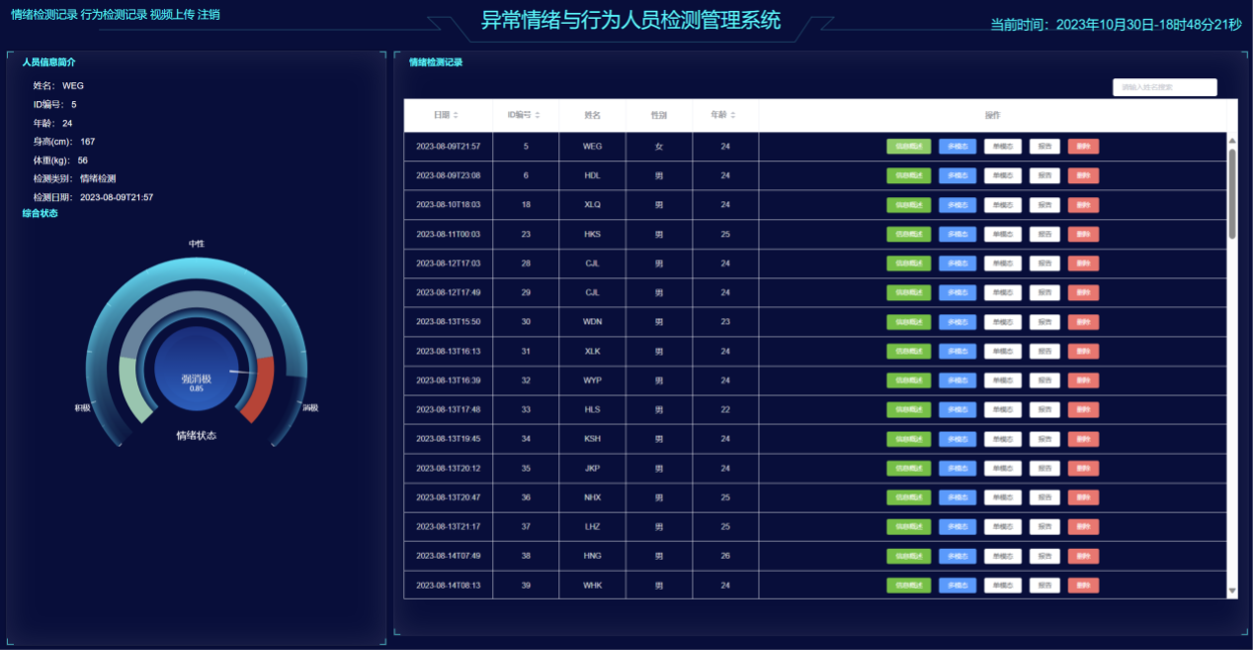
\includegraphics[width=1\textwidth]{Fig3.png}
\caption{Emotion Detection Record.}\label{fig3}
\end{figure}

The information preview function enables users to swiftly peruse basic details of each emotion detection record, such as time, subject, and emotion type, facilitating an initial understanding of the data. The data visualization analysis, a highlight of this interface, transforms complex emotional data into easily comprehensible visual information through charts and graphics, aiding in-depth analysis of various dimensions and patterns in emotion detection. The report generation feature offers a convenient way to produce detailed emotion detection reports as needed, encompassing thorough data analyses and potentially expert interpretations and recommendations, ideal for professional or extensive research purposes. The information deletion and search functionalities provide robust data management, allowing users to quickly locate specific records and maintain data relevance and timeliness.

The emotion detection data visualization analysis interface, as shown in Figures \ref{fig4} and \ref{fig5}, employs data from multiple sources such as facial expressions, voice, text, and multimodal inputs for a comprehensive analysis and assessment of subjects' emotional states. This interface not only reflects the subject's current emotional state in real-time but also reveals trends in emotional changes and the proportion of different emotion categories over time.

In facial expression analysis, the system uses advanced facial recognition technology to identify and interpret subtle changes in the subject's expressions. Voice analysis infers emotional changes through features like tone and speech rate. Text analysis, utilizing natural language processing, captures underlying emotional cues in written or spoken content.

Most crucially, multimodal emotion analysis integrates data from expressions, voice, and text for a more thorough analysis of emotional states, offering more accurate and comprehensive results than single data sources.

\begin{figure}[h]%
\centering
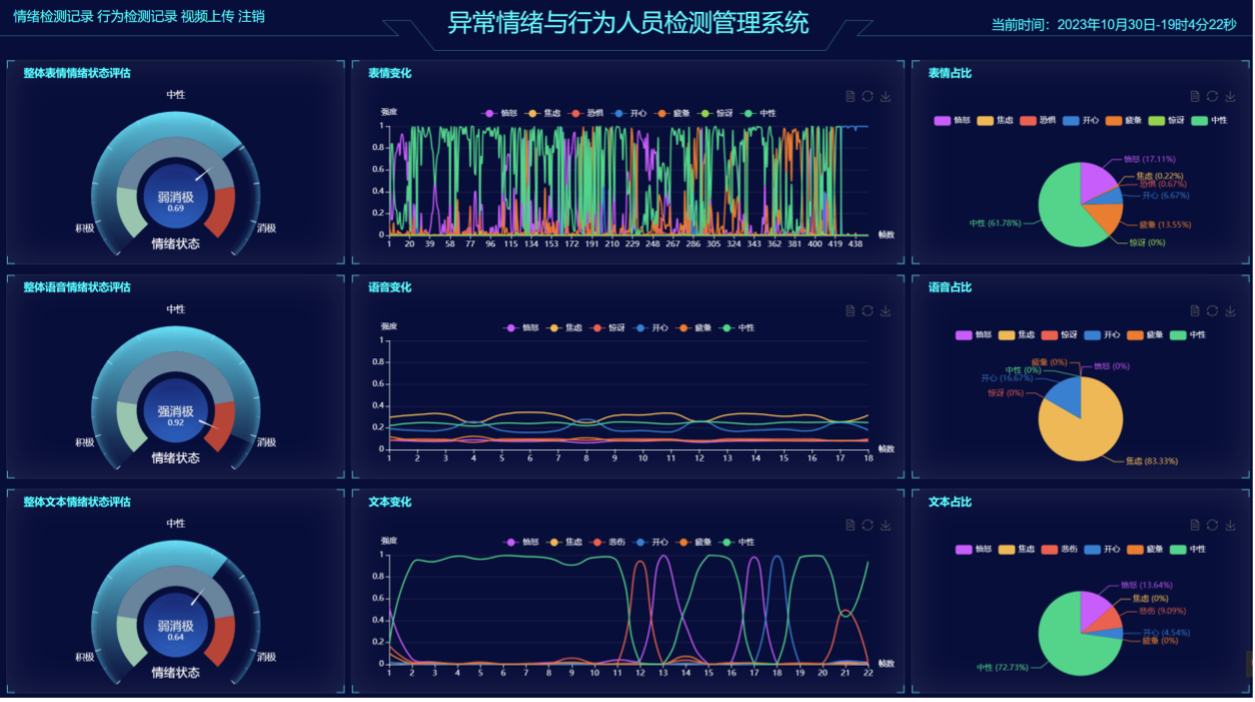
\includegraphics[width=1\textwidth]{Fig4.png}
\caption{Visual Analysis of Emotion Recognition Results in Facial Expression, Voice, and Text Modalities.}\label{fig4}
\end{figure}

\begin{figure}[h]%
\centering
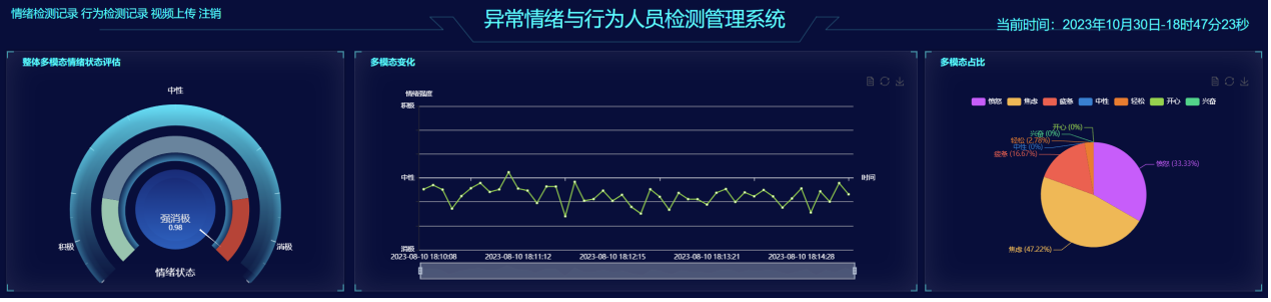
\includegraphics[width=1\textwidth]{Fig5.png}
\caption{Visual Analysis of Multimodal Emotion Recognition Results.}\label{fig5}
\end{figure}

As demonstrated in Figure \ref{fig6}, the behavior detection data visualization analysis interface of this project aims to comprehensively assess the behavioral states of subjects. The interface, with its intuitive charts and data presentations, facilitates a deep understanding of subjects' behavioral characteristics and their trends over time.

Key functionalities include a holistic analysis of subjects' behavior, encompassing not only current behavior patterns but also trends over time. Tracking and analyzing this data offers insights into the trajectory of individual behaviors, allowing for the timely identification of any anomalous or noteworthy patterns.

The interface also emphasizes the analysis of the proportion of various behavior types, presented through various chart forms such as pie and bar graphs. These visual representations effectively show the weight of different behavior patterns in the total behavior of subjects. This categorization and comparison aid in better understanding individuals' behavioral tendencies and the diversity and complexity of behavior patterns in different contexts.


\begin{figure}[h]%
\centering
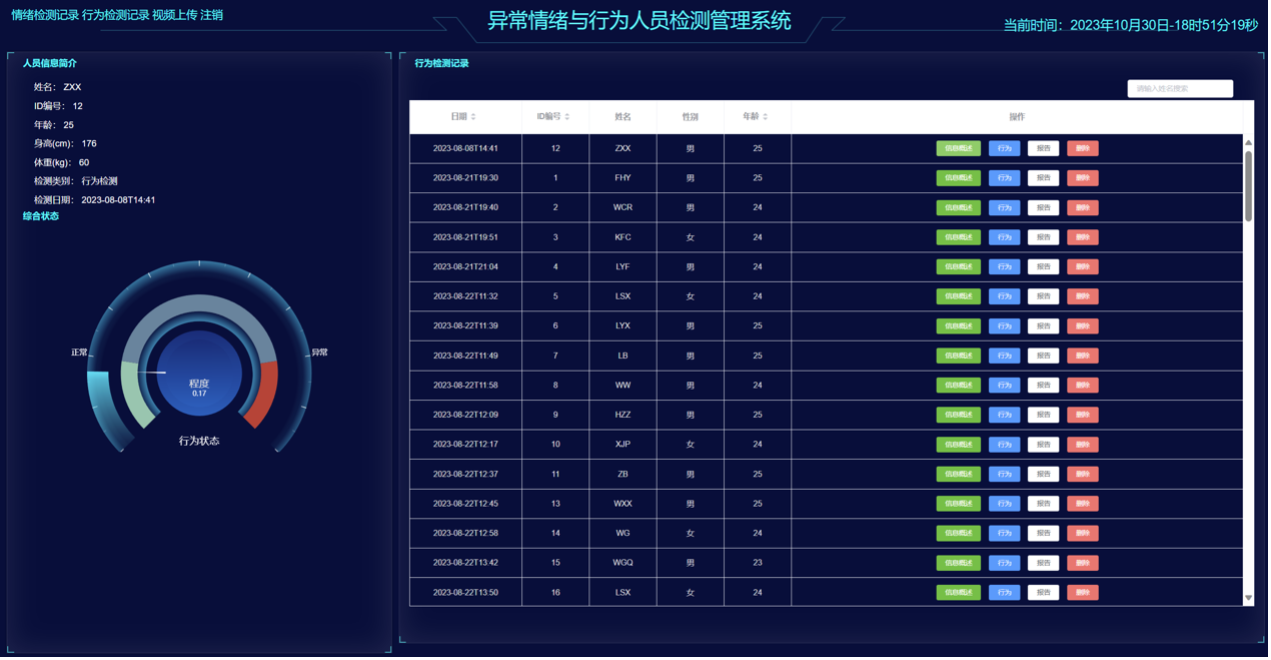
\includegraphics[width=1\textwidth]{Fig6.png}
\caption{Behavior Monitoring Record.}\label{fig6}
\end{figure}


\begin{figure}[!h]%
\centering
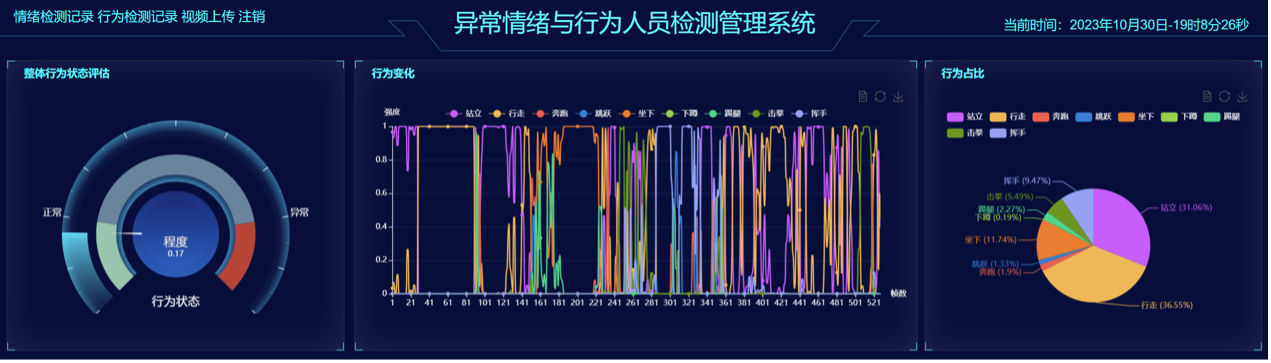
\includegraphics[width=1\textwidth]{Fig7.png}
\caption{Visual Analysis of Emotion Recognition Results from Behavioral Modalities.}\label{fig7}
\end{figure}
\begin{figure}[!h]%
\centering
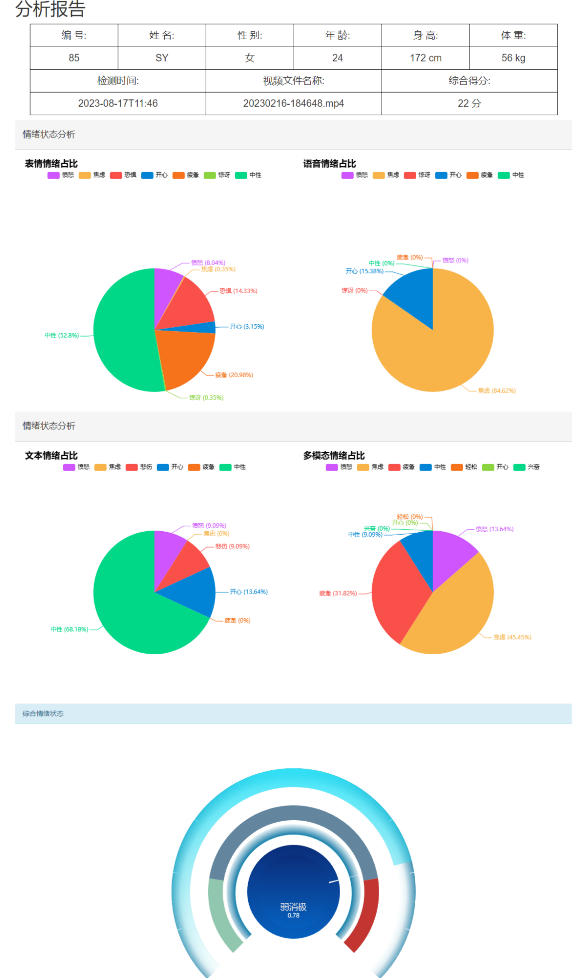
\includegraphics[width=0.7\textwidth]{Fig8.png}
\caption{Emotional Assessment Report.}\label{fig8}
\end{figure}


\begin{figure}[!h]%
\centering
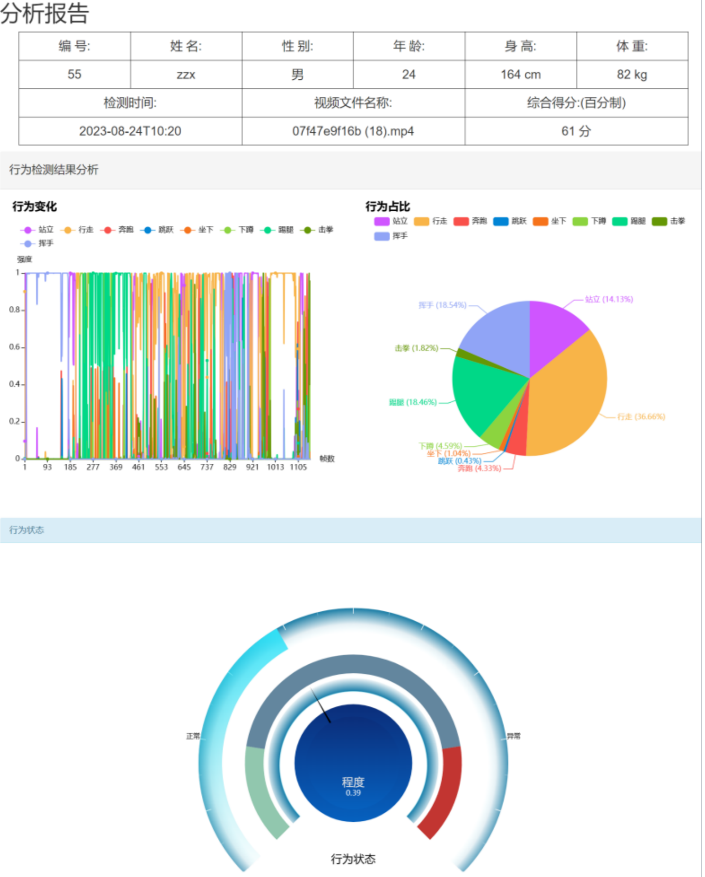
\includegraphics[width=0.7\textwidth]{Fig9.png}
\caption{Behavior Assessment Report.}\label{fig9}
\end{figure}

Figure \ref{fig8} displays the emotional state assessment report, focusing on analyzing users' emotional fluctuations and characteristics, encompassing a range of emotions including happiness, sadness, anger, and surprise. By delving into users' emotional data across different times and contexts, the report reveals patterns and traits of emotional changes, offering personalized emotional management advice.

Figure \ref{fig9}  presents the behavioral state assessment report, emphasizing users' behavior patterns, including activity frequency and habits. This comprehensive observation and analysis of user behavior not only reflect habitual actions but also uncover potential patterns, aiding users in better understanding their behavior and making necessary adjustments.

Together, these reports provide a thorough psychological and behavioral assessment of the user. Employing scientific data analysis and artificial intelligence, the system aims to enhance self-awareness, facilitating improved self-management and mental well-being in daily life and work.




\subsection{System Application Analysis}

Based on the research content discussed above, here are several typical applications of the system:

Interrogation Analysis: In the judicial system, accurate assessment of emotions and behaviors during interrogations is crucial. This system can analyze the interviewee's voice and facial expressions to identify their true emotions and potential deceptive behaviors. With real-time analysis of the interviewee’s behavioral patterns, interrogators can better judge the reliability of testimonies, thereby enhancing the efficiency and accuracy of interrogations.

Recommendation Systems: In e-commerce and content recommendation platforms, users' emotional states significantly influence their decision-making processes. By integrating this system, platforms can analyze users' emotional responses in real-time, allowing for more precise product or content recommendations. This enhances user experience and optimizes marketing strategies for businesses.

Medical Monitoring: In medical settings, patient emotion management has a significant impact on treatment outcomes. The system can be used to monitor patients' emotional changes, especially in mental health treatment, serving as an auxiliary tool for therapeutic effectiveness assessment. Additionally, it can assist doctors in remotely identifying patients' emotional and behavioral states in telemedicine services.

Campus Safety: Schools are critical environments for adolescent development, where students' emotional states directly affect their learning and social interactions. This system can help educators monitor potential abnormal behaviors and emotional fluctuations in student groups, timely identifying issues like bullying, excessive stress, or other mental health problems, and thereby take appropriate measures to ensure campus safety.

\section{Conclusion and Future Research}

In the current wave of artificial intelligence and machine learning research, the development and application of comprehensive human emotion and behavior assessment systems have become a hot topic in interdisciplinary research. The system developed in this study, based on deep learning and image processing technologies, achieves efficient and accurate multimodal emotion recognition and behavior identification, significantly enhancing applicability and accuracy in complex environments. Experimental validation shows that this system excels in emotion and behavior recognition, proving the necessity and effectiveness of multimodal analysis. The end-to-end emotion and behavior recognition system proposed in this study not only fills a gap in existing technology but also demonstrates immense potential in practical applications such as recommendation systems and abnormal emotion diagnosis. Importantly, the open-source code provides a valuable resource for the research and development community, contributing to the continuous progress and development in the field of affective computing. Additionally, our designed emotion state assessment and behavior state reports provide users with comprehensive and in-depth psychological and behavioral analysis, aiding in the optimization of individual emotion management and behavior adjustment, and offering scientific data support and decision-making reference for professionals in related fields. These comprehensive assessment reports enable users to more profoundly understand and grasp their own emotional fluctuations and behavioral patterns.

However, in practical application, we have also identified several limitations of the system: In multi-person emotion recognition, the system still faces challenges with insufficient recognition accuracy. When facing multi-person emotion analysis, issues such as mutual occlusion and expression confusion may reduce recognition efficiency, impacting the overall performance of the system. This challenge requires further optimization of algorithm models in future research to enhance the system's capability to recognize emotions in complex multi-person scenarios. The system's real-time performance also needs improvement. Although our model can process large amounts of data and provide accurate analysis, it does not fully meet the high real-time requirements in rapidly changing real-time scenarios. Especially in applications demanding quick responses, such as emergency medical aid or public safety monitoring, this limitation might affect decision-making timeliness. Despite providing open-source code to promote technology sharing and community collaboration, the complexity of the system requires users to have a certain technical background for effective utilization. This barrier might limit the system's widespread use among non-technical users, and our next step is to integrate our model to be more easily deployable. Although our emotion state assessment and behavior state reports can provide users with in-depth analysis and recommendations, automated systems cannot fully replace the meticulous observation and judgment of professionals. Therefore, in practical applications, we suggest combining the expertise and knowledge of professionals to achieve the best assessment results.

\section*{Declarations}
\begin{itemize}
\item Conflict of interest/Competing interests: There is no conflict of interest in our work.
\item This work was supported by National Natural Science Foundation of China(61771299)
\item Authors' contributions: Wang Rui and Zhu Xianxun contributed the central idea, analyzed most of the data and wrote the first draft of the paper. The rest of the authors devoted themselves to perfecting these ideas, made additional analysis, and finally completed this paper.
\end{itemize}

\begin{thebibliography}{99}

%% \bibitem{label}
%% Text of bibliographic item
\bibitem{ref1} Liu, J., Ang, M. C., Chaw, J. K., Kor, A. L., \& Ng, K. W. (2023). Emotion assessment and application in human-computer interaction interface based on backpropagation neural network and artificial bee colony algorithm. Expert Systems with Applications, 120857.
\bibitem{ref2} Ezzameli, K., \& Mahersia, H. (2023). Emotion recognition from unimodal to multimodal analysis: A review. Information Fusion, 101847.
\bibitem{ref3} Singh, P., Srivastava, R., Rana, K. P. S., \& Kumar, V. (2021). A multimodal hierarchical approach to speech emotion recognition from audio and text. Knowledge-Based Systems, 229, 107316.
\bibitem{ref4} Cooper, J. O., Heron, T. E., \& Heward, W. L. (2020). Applied behavior analysis. Pearson UK.
\bibitem{ref5} Germani, F., \& Biller-Andorno, N. (2021). The anti-vaccination infodemic on social media: A behavioral analysis. PloS one, 16(3), e0247642.
\bibitem{ref6} Fei, Z., Yang, E., Li, D. D. U., Butler, S., Ijomah, W., Li, X., \& Zhou, H. (2020). Deep convolution network based emotion analysis towards mental health care. Neurocomputing, 388, 212-227.
\bibitem{ref7} Kleinschmidt, M., \& Gelbart, D. (2002, September). Improving word accuracy with Gabor feature extraction. In Interspeech.
\bibitem{ref8} Rahim, M. A., Hossain, M. N., Wahid, T., \& Azam, M. S. (2013). Face recognition using local binary patterns (LBP). Global Journal of Computer Science and Technology, 13(4), 1-8.
\bibitem{ref9} Dino, H. I., \& Abdulrazzaq, M. B. (2019, April). Facial expression classification based on SVM, KNN and MLP classifiers. In 2019 International Conference on Advanced Science and Engineering (ICOASE) (pp. 70-75). IEEE.
\bibitem{ref10} Mensah, J. A., Appati, J. K., Boateng, E. K., Ocran, E., \& Asiedu, L. (2024). FaceNet recognition algorithm subject to multiple constraints: Assessment of the performance. Scientific African, 23, e02007.
\bibitem{ref11} Al Maruf, A., Khanam, F., Haque, M. M., Jiyad, Z. M., Mridha, F., \& Aung, Z. (2024). Challenges and Opportunities of Text-based Emotion Detection: A Survey. IEEE Access.
\bibitem{ref12} Ameer, I., Bölücü, N., Siddiqui, M. H. F., Can, B., Sidorov, G., \& Gelbukh, A. (2023). Multi-label emotion classification in texts using transfer learning. Expert Systems with Applications, 213, 118534.
\bibitem{ref13} Kang, Y., Yang, X., Zhang, L., Luo, X., Xu, Y., Wang, H., \& Liu, J. (2024). MGMFN: Multi-graph and MLP-mixer fusion network for Chinese social network sentiment classification. Multimedia Tools and Applications, 1-22.
\bibitem{ref14} Ouni, S., Fkih, F., \& Omri, M. N. (2023). A survey of machine learning-based author profiling from texts analysis in social networks. Multimedia Tools and Applications, 1-34.
\bibitem{ref15} Roy, T., Marwala, T., \& Chakraverty, S. (2020). A survey of classification techniques in speech emotion recognition. Mathematical Methods in Interdisciplinary Sciences, 33-48.
\bibitem{ref16} Liu, H., Zheng, X., Wang, Y., Zhang, Y., \& Liu, K. (2021). A Gaussian mixture-hidden Markov model of human visual behavior. Sheng wu yi xue Gong Cheng xue za zhi= Journal of Biomedical Engineering= Shengwu Yixue Gongchengxue Zazhi, 38(3), 512-519.
\bibitem{ref17} Das, A., \& Mohanty, M. N. (2023). Handwritten Odia numeral recognition using combined CNN-RNN. International Journal of Grid and Utility Computing, 14(4), 382-388.
\bibitem{ref18} Wani, T. M., Gunawan, T. S., Qadri, S. A. A., Kartiwi, M., \& Ambikairajah, E. (2021). A comprehensive review of speech emotion recognition systems. IEEE access, 9, 47795-47814.
\bibitem{ref19} Gandhi, A., Adhvaryu, K., Poria, S., Cambria, E., \& Hussain, A. (2023). Multimodal sentiment analysis: A systematic review of history, datasets, multimodal fusion methods, applications, challenges and future directions. Information Fusion, 91, 424-444.
\bibitem{ref20} Gaw, N., Yousefi, S., \& Gahrooei, M. R. (2022). Multimodal data fusion for systems improvement: A review. IISE Transactions, 54(11), 1098-1116.
\bibitem{ref21} Kalamkar, S. (2023). Multimodal image fusion: A systematic review. Decision Analytics Journal, 100327.
\bibitem{ref22} Tang, Q., Liang, J., \& Zhu, F. (2023). A comparative review on multi-modal sensors fusion based on deep learning. Signal Processing, 109165.
\bibitem{ref23} Pandeya, Y. R., \& Lee, J. (2021). Deep learning-based late fusion of multimodal information for emotion classification of music video. Multimedia Tools and Applications, 80, 2887-2905.
\bibitem{ref24} Jiang, Y., Li, W., Hossain, M. S., Chen, M., Alelaiwi, A., \& Al-Hammadi, M. (2020). A snapshot research and implementation of multimodal information fusion for data-driven emotion recognition. Information Fusion, 53, 209-221.
\bibitem{ref25} Wen, J., Jiang, D., Tu, G., Liu, C., \& Cambria, E. (2023). Dynamic interactive multiview memory network for emotion recognition in conversation. Information Fusion, 91, 123-133.
\bibitem{ref26} Bin, Y., Chen, Z. M., Wei, X. S., Chen, X., Gao, C., \& Sang, N. (2020). Structure-aware human pose estimation with graph convolutional networks. Pattern Recognition, 106, 107410.
\bibitem{ref27} Xin, W., Liu, R., Liu, Y., Chen, Y., Yu, W., \& Miao, Q. (2023). Transformer for Skeleton-based action recognition: A review of recent advances. Neurocomputing.
\bibitem{ref28} Yang, H., Guo, L., Wu, X., \& Zhang, Y. (2022). Scale-aware attention-based multi-resolution representation for multi-person pose estimation. Multimedia Systems, 28(1), 57-67.
\bibitem{ref29} Yang, Y., Li, L., Liu, Z., \& Liu, G. (2020). Abnormal behavior recognition based on spatio-temporal context. Journal of Information Processing Systems, 16(3), 612-628.
\bibitem{ref30} Alafif, T., Alzahrani, B., Cao, Y., Alotaibi, R., Barnawi, A., \& Chen, M. (2022). Generative adversarial network based abnormal behavior detection in massive crowd videos: A Hajj case study. Journal of Ambient Intelligence and Humanized Computing, 13(8), 4077-4088.
\bibitem{ref31} Logan, B. (2000, October). Mel frequency cepstral coefficients for music modeling. In Ismir (Vol. 270, No. 1, p. 11).
\bibitem{ref32} Xiao, Y., Wang, D., \& Hou, L. (2019). Unsupervised emotion recognition algorithm based on improved deep belief model in combination with probabilistic linear discriminant analysis. Personal and Ubiquitous Computing, 23, 553-562.
\bibitem{ref33} Zheng, H., \& Yang, Y. (2019, July). An improved speech emotion recognition algorithm based on deep belief network. In 2019 IEEE international conference on power, intelligent computing and systems (ICPICS) (pp. 493-497). IEEE.
\bibitem{ref34} Gao, Y., Morioka, N., Zhang, Y., \& Chen, N. (2023, December). E3 TTS: Easy End-to-End Diffusion-Based Text To Speech. In 2023 IEEE Automatic Speech Recognition and Understanding Workshop (ASRU) (pp. 1-8). IEEE.
\bibitem{ref35} Yun, H. I., \& Park, J. S. (2023). End-to-end emotional speech recognition using acoustic model adaptation based on knowledge distillation. Multimedia Tools and Applications, 1-18.
\bibitem{ref36} Acheampong, F. A., Nunoo-Mensah, H., \& Chen, W. (2021). Transformer models for text-based emotion detection: a review of BERT-based approaches. Artificial Intelligence Review, 1-41.
\bibitem{ref37} Jiang, Y., Li, W., Hossain, M. S., Chen, M., Alelaiwi, A., \& Al-Hammadi, M. (2020). A snapshot research and implementation of multimodal information fusion for data-driven emotion recognition. Information Fusion, 53, 209-221.
\bibitem{ref38} Acheampong, F. A., Nunoo-Mensah, H., \& Chen, W. (2021). Transformer models for text-based emotion detection: a review of BERT-based approaches. Artificial Intelligence Review, 1-41.
\bibitem{ref39} Tejashwini, S. G., \& Aradhana, D. (2023). Revolutionizing sentiment classification: A deep learning approach using self-attention based encoding–decoding transformers with feature fusion. Engineering Applications of Artificial Intelligence, 125, 106730.
\bibitem{ref40} Liu, C., \& Xu, X. (2021). AMFF: A new attention-based multi-feature fusion method for intention recognition. Knowledge-Based Systems, 233, 107525.
\bibitem{ref41} Zhang, Y., Chen, S., Cao, W., Guo, P., Gao, D., Wang, M., ... \& Wang, T. (2021). MFFNet: Multi-dimensional Feature Fusion Network based on attention mechanism for sEMG analysis to detect muscle fatigue. Expert Systems with Applications, 185, 115639.
\bibitem{ref42} Fu, Z., Liu, F., Xu, Q., Fu, X., \& Qi, J. (2024). LMR-CBT: Learning modality-fused representations with CB-transformer for multimodal emotion recognition from unaligned multimodal sequences. Frontiers of Computer Science, 18(4), 184314.
\bibitem{ref43} Hu, R., \& Singh, A. (2021). Unit: Multimodal multitask learning with a unified transformer. In Proceedings of the IEEE/CVF International Conference on Computer Vision(pp. 1439-1449).
\bibitem{ref44} Liang, X., Zou, Y., Zhuang, X., Yang, J., Niu, T., \& Xu, R. (2023). MMATERIC: Multi-Task Learning and Multi-Fusion for AudioText Emotion Recognition in Conversation. Electronics, 12(7), 1534.
\bibitem{ref45} Li, J., Liu, X., Zhang, W., Zhang, M., Song, J., \& Sebe, N. (2020). Spatio-temporal attention networks for action recognition and detection. IEEE Transactions on Multimedia, 22(11), 2990-3001.
\bibitem{ref46} Muhammad, K., Ullah, A., Imran, A. S., Sajjad, M., Kiran, M. S., Sannino, G., \& de Albuquerque, V. H. C. (2021). Human action recognition using attention based LSTM network with dilated CNN features. Future Generation Computer Systems, 125, 820-830.
\bibitem{ref47} Lv, M., Chen, Z., Guo, C., \& Hemalatha, K. L. (2023, March). Multi-modal Interactive Experience Design of Automotive Central Control System. In The International Conference on Cyber Security Intelligence and Analytics(pp. 309-320). Cham: Springer Nature Switzerland.
\bibitem{ref48} Lynch, C., Wahid, A., Tompson, J., Ding, T., Betker, J., Baruch, R., ... \& Florence, P. (2023). Interactive language: Talking to robots in real time. IEEE Robotics and Automation Letters.
\bibitem{ref49} Zhang, J., Yin, Z., Chen, P., \& Nichele, S. (2020). Emotion recognition using multi-modal data and machine learning techniques: A tutorial and review. Information Fusion, 59, 103-126.
\bibitem{ref50} Ravanelli, M., Zhong, J., Pascual, S., Swietojanski, P., Monteiro, J., Trmal, J., \& Bengio, Y. (2020, May). Multi-task self-supervised learning for robust speech recognition. In ICASSP 2020-2020 IEEE International Conference on Acoustics, Speech and Signal Processing (ICASSP) (pp. 6989-6993). IEEE.
\bibitem{ref51} Amal, V. S., Suresh, S., \& Deepa, G. (2022). Real-time emotion recognition from facial expressions using convolutional neural network with Fer2013 dataset. In Ubiquitous Intelligent Systems: Proceedings of ICUIS 2021 (pp. 541-551). Springer Singapore.
\bibitem{ref52} Liu, B., Xu, X., \& Zhang, Y. (2020). Offline handwritten Chinese text recognition with convolutional neural networks. arXiv preprint arXiv:2006.15619.
\bibitem{ref53} Wang, D., \& Zhang, X. (2015). Thchs-30: A free chinese speech corpus. arXiv preprint arXiv:1512.01882.
\bibitem{ref54} Peng, S., Zeng, R., Liu, H., Chen, G., Wu, R., Yang, A., \& Yu, S. (2021). Emotion classification of text based on BERT and broad learning system. In Web and Big Data: 5th International Joint Conference, APWeb-WAIM 2021, Guangzhou, China, August 23–25, 2021, Proceedings, Part I 5 (pp. 382-396). Springer International Publishing.
\bibitem{ref55} Lin, T. Y., Maire, M., Belongie, S., Hays, J., Perona, P., Ramanan, D., ... \& Zitnick, C. L. (2014). Microsoft coco: Common objects in context. In Computer Vision–ECCV 2014: 13th European Conference, Zurich, Switzerland, September 6-12, 2014, Proceedings, Part V 13 (pp. 740-755). Springer International Publishing.
\bibitem{ref56} Nan, Y., Ju, J., Hua, Q., Zhang, H., \& Wang, B. (2022). A-MobileNet: An approach of facial expression recognition. Alexandria Engineering Journal, 61(6), 4435-4446.
\bibitem{ref57} Chen, Y., Wang, J., Chen, S., Shi, Z., \& Cai, J. (2019, December). Facial motion prior networks for facial expression recognition. In 2019 IEEE Visual Communications and Image Processing (VCIP) (pp. 1-4). IEEE.
\bibitem{ref58} Li, B., Li, R., \& Lima, D. (2021). Facial expression recognition via ResNet-18. In Multimedia Technology and Enhanced Learning: Third EAI International Conference, ICMTEL 2021, Virtual Event, April 8–9, 2021, Proceedings, Part II 3 (pp. 290-303). Springer International Publishing.
\bibitem{ref59} Ghofrani, A., Toroghi, R. M., \& Ghanbari, S. (2019, February). Realtime face-detection and emotion recognition using mtcnn and minishufflenet v2. In 2019 5th Conference on Knowledge Based Engineering and Innovation (KBEI) (pp. 817-821). IEEE.
\bibitem{ref60} Kalyta, O., Barmak, O., Radiuk, P., \& Krak, I. (2023). Facial Emotion Recognition for Photo and Video Surveillance Based on Machine Learning and Visual Analytics. Applied Sciences, 13(17), 9890.
\bibitem{ref61} Sarker, M. K., Alam, K. M. R., \& Arifuzzaman, M. (2014, May). Emotion recognition from speech based on relevant feature and majority voting. In 2014 International Conference on Informatics, Electronics \& Vision (ICIEV)(pp. 1-5). IEEE.
\bibitem{ref62} Chen, L., Su, W., Feng, Y., Wu, M., She, J., \& Hirota, K. (2020). Two-layer fuzzy multiple random forest for speech emotion recognition in human-robot interaction. Information Sciences, 509, 150-163.
\bibitem{ref63} Wu, T., Wang, L., \& Zhang, J. (2023, November). CM-TCN: Channel-Aware Multi-scale Temporal Convolutional Networks for Speech Emotion Recognition. In International Conference on Neural Information Processing (pp. 459-476). Singapore: Springer Nature Singapore.
\bibitem{ref64} Teng, Z., Ren, F., \& Kuroiwa, S. (2007, August). Emotion recognition from text based on the rough set theory and the support vector machines. In 2007 International Conference on Natural Language Processing and Knowledge Engineering (pp. 36-41). IEEE.
\bibitem{ref65} Shan, D., \& Li, H. (2023). Group Emotion Recognition for Weibo Topics Based on BERT with TextCNN. American Journal of Information Science and Technology, 7(3), 95-100.
\bibitem{ref66} Batbaatar, E., Li, M., \& Ryu, K. H. (2019). Semantic-emotion neural network for emotion recognition from text. IEEE access, 7, 111866-111878.
\bibitem{ref67} Ye, Z., Zuo, T., Chen, W., Li, Y., \& Lu, Z. (2023). Textual emotion recognition method based on ALBERT-BiLSTM model and SVM-NB classification. Soft Computing, 27(8), 5063-5075.
\bibitem{ref68} Peng, S., Zeng, R., Liu, H., Chen, G., Wu, R., Yang, A., \& Yu, S. (2021). Emotion classification of text based on BERT and broad learning system. In Web and Big Data: 5th International Joint Conference, APWeb-WAIM 2021, Guangzhou, China, August 23–25, 2021, Proceedings, Part I 5 (pp. 382-396). Springer International Publishing.
\bibitem{ref69} Liang, P. P., Zadeh, A., \& Morency, L. P. (2018, October). Multimodal local-global ranking fusion for emotion recognition. In Proceedings of the 20th ACM International Conference on Multimodal Interaction (pp. 472-476).
\bibitem{ref70} Liang, X., Zou, Y., Zhuang, X., Yang, J., Niu, T., \& Xu, R. (2023). MMATERIC: Multi-Task Learning and Multi-Fusion for AudioText Emotion Recognition in Conversation. Electronics, 12(7), 1534.
\bibitem{ref71} Li, Y. K., Meng, Q. H., Wang, Y. X., \& Hou, H. R. (2023). MMFN: Emotion recognition by fusing touch gesture and facial expression information. Expert Systems with Applications, 228, 120469.
\bibitem{ref72} Sun, J., Han, S., Ruan, Y. P., Zhang, X., Zheng, S. K., Liu, Y., ... \& Li, T. (2023, July). Layer-wise fusion with modality independence modeling for multi-modal emotion recognition. In Proceedings of the 61st Annual Meeting of the Association for Computational Linguistics (Volume 1: Long Papers) (pp. 658-670).
\bibitem{ref73} Pan, H., Li, Y., \& Zhao, D. (2021). Recognizing human behaviors from surveillance videos using the SSD algorithm. The Journal of Supercomputing, 77, 6852-6870.
\bibitem{ref74} Gangodkar, D., \& Vimal, V. (2021). Video Object Detection Using Densenet-Ssd. Webology, 18(5), 3256-3261.
\bibitem{ref75} Hung, P. D., \& Su, N. T. (2021). Unsafe construction behavior classification using deep convolutional neural network. Pattern Recognition and Image Analysis, 31(2), 271-284.
\bibitem{ref76} Carreira, J., \& Zisserman, A. (2017). Quo vadis, action recognition? a new model and the kinetics dataset. In proceedings of the IEEE Conference on Computer Vision and Pattern Recognition (pp. 6299-6308).




\end{thebibliography}
\end{document}
\endinput
%%
%% End of file `elsarticle-template-num.tex'.
